%!TEX root = ../Thesis.tex

\section{Skip-gram}

The Skip-gram model tries to learn the meaning of words by its context. Specifically it tries to predict the surrounding words given a single input word.

The Skip-gram model does this by encoding the input word using 1-of-V encoding where $V$ is the vocabulary size. This means that each word is represented as an indicator vector, where the vector represent a single word from a given vocabulary. The vocabulary is typically defined using the $V$ most common word in the text corpus. \marginnote{\vspace{-1.5cm}\textbf{corpus}: \\ collection of documents}
\begin{figure}[h]
\begin{equation*}
\begin{aligned}
\text{twinkle}: \left[1, 0, 0, 0, \cdots \right] \\
\text{twinkle}: \left[1, 0, 0, 0, \cdots \right] \\
\text{little}: \left[0, 1, 0, 0, \cdots \right] \\
\text{star}: \left[0, 0, 1, 0, \cdots \right]
\end{aligned}
\end{equation*}
\caption{Example of 1-of-V encoding on the sentence ``twinkle twinkle little star''}
\end{figure}

Each of these word representations are then transformed into a lower dimensional space (latent representation). In this space, words with same meaning should be close to each other. The position of each word should also contain a higher semantic meaning, such that for example $f(King) - f(Man) + f(Female) \approx f(Queen)$ \cite{word2vec-comparing}. Here $f$ is the transformation function from the input space to the latent representation.

The model is trained such that the surrounding words can be predicted from this latent representation. See Figure \ref{fig:theory:skip-gram:graph} for a graphical overview. An important detail about this model, is that the order of the words within the considered text window have no effect on the training. Thus all surrounding are assumed to having approximately the same meaning.

\begin{figure}[h]
	\centering
	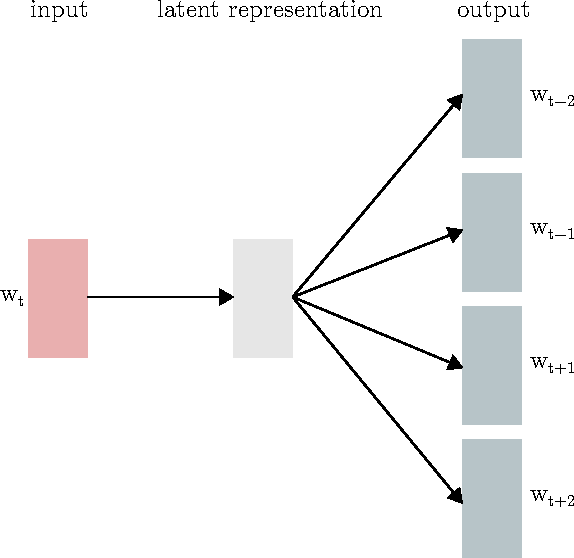
\includegraphics[scale=0.7]{theory/skip-gram-graph}
	\caption{Visualization of the Skip-gram model. Given a single input word it tries to predict the surrounding words. From this the latent representation is learned.}
	\label{fig:theory:skip-gram:graph}
\end{figure}

\subsection{The likelihood function}
The Skip-gram model is optimized by maximum-likelihood. Given a corpus with $\mathcal{D}$ documents where each document have $T_d$ words, the likelihood function is calculated using the conditional probability of observing the surrounding words ($w_{d, t + \ell}$) given the input words ($w_{d, t}\ , t \in [1, T_d]$).
\begin{equation}
\prod_{d = 1}^{\mathcal{D}} \prod_{t = 1}^{T_d} \prod_{\ell} p(w_{d, t + \ell} | w_{d, t})
\label{eq:theory:skipgram:full-likelihood}
\end{equation}

The details about which document there currently is used, are typically omitted from the expressions. Thus equation \eqref{eq:theory:skipgram:full-likelihood} becomes:
\begin{equation}
\prod_{t = 1}^{T} \prod_{\ell} p(w_{t + \ell} | w_{t})
\end{equation}

Since words closer to $w_t$ are expected to be more related to that word, the near surrounding words are weighted higher. This is not modelled by explicit weights, but instead by letting $\ell \in [-R, R] \setminus \{ 0 \}$ where $R \sim U[1, C]$ \cite{word2vec-comparing}.

As usual the negative log is used to get the loss function:
\begin{equation}
\mathcal{L} = - \sum_{t = 1}^T \sum_{\ell} \ln( p(w_{t + \ell} | w_t) )
\end{equation}

In \cite{word2vec-details} a likelihood function is used (sign is flipped) and it is averaged over time ($\sfrac{1}{T}$ is multiplied).

\subsection{Forward pass}
The conditional probability $p(w_{t + \ell} | w_t)$ is calculated using a log-linear model. This is best explained by considering a neural network, with a single hidden layer and no non-linear units ($\theta(a) = a$).

\begin{figure}[H]
	\centering
	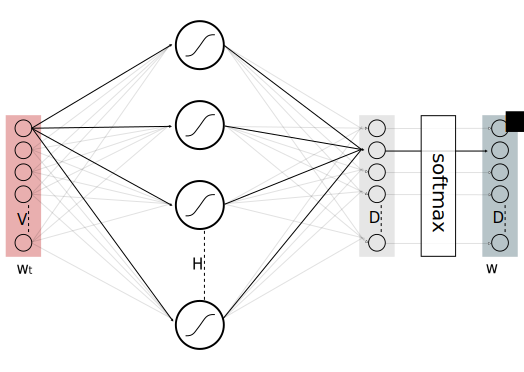
\includegraphics[scale=0.7]{theory/skip-gram-network}
	\caption{Visualization of a single pass though the Skip-gram network.}
	\label{fig:theory:skipgram:network}
\end{figure}

As seen in Figure \ref{fig:theory:skipgram:network} the Skip-gram model is really just a very simple feed forward neural network. The forward equations for this kind of network have already been covered in section \ref{sec:theory:ffnn}, thus deriving the forward equation for the Skip-gram model is just a simple exercise of using that theory. 

By setting $h_0 = K = V$, $h_1 = D$ and defining $\{x^t_i\}_{i=1}^V$ as the indicator vector for the word $w_t$, the forward pass becomes:
\begin{equation}
\begin{aligned}
b_{h_1}^t = a_{h_1}^t &= \sum_{i = 1}^V w_{i, h_1} x_i^t, && \forall h_1 \in [1, D] \\
a_{k}^t = a_{h_2}^t &= \sum_{h_1 = 1}^{D} w_{h_1, h_2} b_{h_1}^t, && \forall h_2 \in [1, V] \\
y_k^t &= \frac{\exp(a_k^t)}{\sum_{k'=1}^V \exp(a_{k'}^t)}, && \forall k \in [1, V]
\end{aligned}
\label{eq:theory:skipgram:forwardpass}
\end{equation}

It is possible to reformulate the \eqref{eq:theory:skipgram:forwardpass} equations, such that they appear as in \cite{word2vec-details}. However it is a bit convoluted as it requires using vector notation and using a trick where subscript selection is done by knowing that $x^t$ is an indicator vector. Thus that won't be covered here, but see Appendix \ref{appendix:skipgram} for how it can be done.

Calculating $y_k^t$ is problematic since it contains a sum over all words in the vocabulary. In the Skip-gram model the vocabulary can be of size $10^5$ to $10^7$ \cite{word2vec-details}. This is why \cite{word2vec-comparing, word2vec-details, word2vec-explained} uses an approximation in form of either \textit{hierarchical softmax} or \textit{negative-sampling}. These approximations will not be discussed here, but are worth considering as they will reduce the computational complexity from $\mathcal{O}(V)$ to $\mathcal{O}(\ln_2(V))$ \cite{word2vec-comparing}.

\subsection{Backward pass}

Deriving the backward pass have similarly been covered in section \ref{sec:theory:ffnn}. First step is to express $\ln( p(w_{t + \ell} | w_t) )$ using a target vector, this vector will be denoted $t^{t+\ell}$ for the word $w_{t + \ell}$:
\begin{equation}
\mathcal{L} =  - \sum_{t = 1}^T \sum_{\ell} \ln( p(w_{t + \ell} | w_t)) =  - \sum_{t = 1}^T \sum_{\ell} \sum_{k=1}^V t_k^{t+\ell} \ln(y_k^t)
\end{equation}

The loss function is a little difference compared to that in section \ref{sec:theory:ffnn}. However because it maintains a linear relation to the loss function used in section \ref{sec:theory:ffnn}, this doesn't matter.
\begin{equation}
\begin{aligned}
\frac{\partial \mathcal{L}}{\partial w_{h_{\ell-1}, h_\ell}} = \sum_{t = 1}^T \sum_{\ell} \frac{\partial}{\partial w_{h_{\ell-1}, h_\ell}} \left(- \sum_{k=1}^V t_k^{t+\ell} \ln(y_k^t)\right), && \forall \ell \in [1, L + 1]
\end{aligned}
\end{equation}

Now it is just a matters of using the method covered in section \ref{sec:theory:ffnn}. First the $\delta_{h_\ell}$ values are calculated. To denote the time and lag a superscript is added:
\begin{equation}
\begin{aligned}
\delta_{h_1}^{t, t + \ell} &= \sum_{h_2=1}^{H_2} \delta_{h_2}^{t, t + \ell} w_{h_1, h_2}, && h_1 \in [1, D] \\
\delta_{h_2}^{t, t + \ell} = \delta_{k}^{t, t + \ell} &= y_k^t - t_k^{t+\ell}, && k \in [1, V]
\end{aligned}
\end{equation}

After the $\delta_{h_\ell}^{t, t+\ell}$ values are calculated, the weight derivatives can be calculated:
\begin{equation}
\begin{aligned}
\frac{\partial \mathcal{L}}{\partial w_{h_{0}, h_1}}= \sum_{t = 1}^T \sum_{\ell} \delta_{h_1}^{t, t + \ell} x_{h_0}^t, && \forall h_0 \in [1, V], h_1 \in [1, D] \\
\frac{\partial \mathcal{L}}{\partial w_{h_{1}, h_2}}= \sum_{t = 1}^T \sum_{\ell} \delta_{h_2}^{t, t + \ell} b_{h_1}^t, && \forall h_1 \in [1, D], h_2 \in [1, V]
\end{aligned}
\end{equation}
